\documentclass[a4paper,11pt]{article}
\usepackage[T1]{fontenc}
\usepackage[utf8]{inputenc}
\usepackage{lmodern}
\usepackage{graphicx}
\usepackage{listings}
\usepackage{amsmath}

\title{Trabajo Practico Algoritmos}
\author{Alan Rodriguez}

\begin{document}

\maketitle
\tableofcontents


\begin{abstract}
\end{abstract}

\section{Algoritmo goloso para el problema del viajante de comercio}

\section*{Heuristica}
El camino se relaizará eligiendo el vecino mas cercano (arista de menor peso)

\section*{Pasos a seguir}
\begin{itemize}
  \item Arrancamos de un nodo.
  \item lo marcamos como visitado.
  \item elegimos la arista de menor peso.
  \item no se puede volver a elegir un nodo ya visitado.
  \item repetir hasta visitar todos los nodos.
\end{itemize}
\begin{figure}
  \begin{center}
    \includegraphics{grafo.jpg}
    \caption{Grafo No Dirigido Completo}
    \label{fig:}
  \end{center}
\end{figure}

\begin{description}
  \item [$V = \{ 1,2,3,4\} $]
  \item [$E = \{ (1,2),(1,3),(1,4),(2,3),(2,4),(3,4)\} $]
\end{description}
 
\section*{Representación} la representacion de grafo elegida es por matriz de adyacencia
\begin{table}[htbp]
\centering
\begin{tabular}{|l|l|l|l|l|}
\hline
&1 & 2 & 3 & 4  \\
\hline
1&-&7&9&8 \\
\hline
2&7&-&10&4 \\
\hline
3&9&10&-&15 \\
\hline
4&8&4&15&- \\
\hline
\end{tabular}
\end{table}

Grafo = $\bigl|\begin{smallmatrix}-&7&9&8\\ 7&-&10&4 \\9&10&-&15 \\8&4&15&- \\\end{smallmatrix}\bigr|$
\begin{lstlisting}
public class GrafoMatriz  {
    public int [][] matAdyacentes;
    ...
  }
      
\end{lstlisting}
\section*{Código en Java}
\begin{itemize}
  \item usare un $nodoActual$ que será el nodo que estamos parados;
  \item  me guardaré la posicion del minimo en $posicionDelMinimo$;
  \item el camino resultante lo guardare en $ caminoRecorrido$
  \item  y para saber que nodo visité usaré $yaLoRecorri$
\end{itemize}

 \lstset{language=Java, breaklines=true, basicstyle=\footnotesize}
\begin{lstlisting}[frame=single]
public static int[] recorridoViajanteDeComercio(GrafoMatriz grafo) {
	int nodoActual = 0;//O (1)
	int posicionDelMinimo=0;//O(1)
	int tamGrafo = grafo.numeroDeVertices();//O(1)
	int [] caminoRecorrido = new int[tamGrafo];//O(1)
	boolean [] yaLoRecorri = new boolean[tamGrafo];//O(1)
	inicializarEnFalso(yaLoRecorri);//O(n)
	inicializarEnCero(caminoRecorrido);//O(n)
	while (!yaLoRecorri[nodoActual]) { //peor de los casos: O(n)
		float[] misAdyacentes = grafo.adyacentesDe(nodoActual);//O(1)
		yaLoRecorri[nodoActual] = true;//O(1)
		insertarEnSiguientePosicionLibre(caminoRecorrido, nodoActual);//peor de los casos O(n)
		float pesoMinimo = grafo.pesoMasAlto(nodoActual);// O(1)
		for (int indice = 0; indice < tamGrafo; indice++) { //todo el if se ejecuta tantas veces como nodos haya O(m)
			if (!yaLoRecorri[indice]) {
				if (misAdyacentes[indice] < pesoMinimo) {
					pesoMinimo = misAdyacentes[indice];
					posicionDelMinimo = indice;
				}
			}
		}
		nodoActual = posicionDelMinimo;//O(1)
	}
	return caminoRecorrido;
} // el while que ejecuta un for define el orden del metodo : O(n.m)
    }
\end{lstlisting}

\section*{Ordenes de Complejidad}
\begin{description}
  \item[inicializar variables int] $O(1)$
  \item[inicializar cada arreglo] $O (n)$ siendo n el tamaño del arreglo
  \item[for dentro del while] $O (n)$ siendo n la cantidad de vertices que tiene el nodo
  \item[while] en el peor de los casos (si se ejecuta siempre) es $O(n)$  siendo n el tamaño del grafo pero tiene un for dentro de $O(n)$ por lo que queda $O(n^{2})$
  \item[tenemos entonces:] $O(n^{2}) + 2 O (n) + O(1)$ por definición no importa el valor de las constantes, lo que crecerá más rápido será $n^{2}$ por lo que es $O(n^{2})$
\end{description}

\section{Algoritmo anterior aleatorio}
\begin{itemize}
  \item Se tendrán en cuenta los primeros mejores caminos.
  \item Se recibirá por parametro una $cotaMinima$ y tendré una variable $cotaMaxima$ que dependerá del tamaño del Grafo.
  \item Usaremos una funcion $Ramdom$ que me dara un número, ese numero será que posicion elijo de los mejores para seguir.
\end{itemize}
 \lstset{language=Java, breaklines=true, basicstyle=\footnotesize}
\begin{lstlisting}[frame=single]
  public static int[] recorridoViajanteDeComercioAleatorio(GrafoMatriz grafo) {
  	int nodoActual = 0;//O (1)
	//int posicionDelMinimo=0;//O(1)
	int tamGrafo = grafo.numeroDeVertices();//O(1)
	int porcentajeDelGrafo = (tamGrafo *10)/100; //O(1)
	if (porcentajeDelGrafo<=0) porcentajeDelGrafo=1;//O(1) // para arreglos muy pequenos que no pueda sacar cierto porcentaje
		int [] caminoRecorrido = new int[tamGrafo];//O(1)
		boolean [] yaLoRecorri = new boolean[tamGrafo];//O(1)
	inicializarEnFalso(yaLoRecorri);//O(n)
	inicializarEnCero(caminoRecorrido);//O(n)
	while (!yaLoRecorri[nodoActual]) { //peor de los casos: O(n)
		float[] misAdyacentes = grafo.adyacentesDe(nodoActual);//O(1) me guardo el peso de las aristas adyacentes al nodo actual
		Candidato[] misCandidatos = new Candidato[tamGrafo];
		yaLoRecorri[nodoActual] = true;//O(1)
		insertarEnSiguientePosicionLibre(caminoRecorrido, nodoActual);//peor de los casos O(n)
		for (int indice = 0; indice < tamGrafo; indice++) {
			if (!yaLoRecorri[indice]) {
				Candidato talCual = new Candidato(misAdyacentes[indice],indice);
				misCandidatos[indice] = talCual;
			}
		else {
			Candidato valorAlto = new Candidato(999999999,indice);
			misCandidatos[indice] = valorAlto;
		}
	}
	Arrays.sort(misCandidatos);
	//double x = (Math.random()*((max-min)+1))+min;
	double sig = Math.random() * ((porcentajeDelGrafo) + 1) + porcentajeDelGrafo;
	int siguiente = (int)sig-1;
	nodoActual = misCandidatos[siguiente].getNumero();//O(1)
	}
	return caminoRecorrido;
}

\end{lstlisting}

\section*{Ordenes de Complejidad}
\begin{description}
  \item[inicializar variables int] $O(1)$
  \item[inicializar cada arreglo] $O (n)$ siendo n el tamaño del arreglo
  \item[for dentro del while] $O (n)$ siendo n la cantidad de vertices que tiene el nodo
  \item[while] en el peor de los casos (si se ejecuta siempre) es $O(n)$  siendo n el tamaño del grafo pero tiene un for dentro de $O(n)$ por lo que queda $O(n^{2})$
  \item[tenemos entonces:] $O(n^{2}) + 2 O (n) + O(1)$ por definición no importa el valor de las constantes, lo que crecerá más rápido será $n^{2}$ por lo que es $O(n^{2})$
\end{description}


\section{Búsqueda local}
\begin{itemize}
  \item la busqueda local recibe una solucion inicial que en principio es la mejor solucion
  \item de esa solucion se buscan los vecinos que son combinaciones de la solucion propuesta, pero no a se realizan grandes cambios (vecinos lejanos)
  \item de haber una solucion optima que mejore a la mejor solucion, se vuelve a correr el algoritmo de busqueda local
\end{itemize}

\lstset{language=Java, breaklines=true, basicstyle=\footnotesize}
\begin{lstlisting}[frame=single]
public static int[] busquedaLocal ( GrafoMatriz grafo) {
	int[] solucionHastaAhora = recorridoViajanteDeComercio(grafo);
	int[] mejorSolucion = solucionHastaAhora.clone();
	float costoOptimo = recorrerElGrafo(grafo,mejorSolucion); // hasta ahora el unico costo que tengo

	List<int[]> vecinos = new ArrayList<>();
	for(int iterador=0; iterador < mejorSolucion.length; iterador++ ){
		int[] vecino = generarVecino(iterador, mejorSolucion.length, solucionHastaAhora);
		vecinos.add(vecino);//agrego al vecino
	}
	for (int[] vecino : vecinos) {
		float otroCosto = recorrerElGrafo(grafo, vecino);
		if (otroCosto <= costoOptimo) {
			costoOptimo = otroCosto;
			mejorSolucion = vecino;
		}
	}
	return mejorSolucion;
}
	

\end{lstlisting}
los vecinos los voy generando haciendo permutaciones
\begin{itemize}
  \item el primero con el segundo
  \item y asi continuo con el siguiente con su consecutivo
  \item el ultimo con el primero 
\end{itemize}
\lstset{language=Java, breaklines=true, basicstyle=\footnotesize}
\begin{lstlisting}[frame=single]
    private static int[] generarVecino(int indice, int tamanioArreglo, int[] laMejorSolucion) {
		int[] vecinoNuevo = laMejorSolucion.clone(); //O(1) //le copio todos los valores
		if (indice < tamanioArreglo-1){ //peor de los caso se ejecuta dos intrucciones de orden 1
		//swappeo el del indice actual y su siguiente
			vecinoNuevo[indice]= laMejorSolucion[indice + 1]; //O(1)
		vecinoNuevo[indice +1] = laMejorSolucion[indice]; //O(1)
		}
		else {
		// swappeo el primero con el ultimo
		vecinoNuevo[indice]= laMejorSolucion[0]; //O(1)
		vecinoNuevo[0] = laMejorSolucion[indice]; //O(1)
		}
		return vecinoNuevo;
	}// ejecuta 3 asignaciones de orden constante -> O(1)
\end{lstlisting}


encotrar la mejor solucion involucra:
\begin{itemize}
  \item de la mejor solucion no debo contar las aristas que no estan mas y que estan en la solucion propuesta
  \item de la solucion propuesta debo sumar aquellas aristas que no tiene la mejor solucion
  
  
\end{itemize}
\section{busqueda local optimizada}
\begin{itemize}
	\item se le mando al algoritmo tres parametros:
	\begin{enumerate}
		\item el grafo
		\item el mejor camino encontrado hasta el momento
		\item y la cantidad maxima que el algoritmo puede llamarse a si mismo buscando la mejor solucion
	\end{enumerate}
	\item el algoritmo busca entre los vecinos del mejor camimo mandado si encuentra uno optimo
	\item si aun quedan iteraciones para realizar se llama recursivamente cambiando los ultimos dos parametros por el vecino optimo y la cantidad de iteraciones menos una		
\end{itemize}

\section{Algoritmo GRASP}
\begin{itemize}
	\item el algoritmo recibe por parametros el grafo, el nombre de archivo de entrada y el nombre de archivo de salida
	\item se crea el grafo correspondiente al archivo de entrada recibido
	\item se crea un nuevo archivo de texto con el nombre de archivo de salida dado
	\item recorremos hamiltoneanamente para obtener una posible solucion
	\item imprimimos en el archivo de salida que hemos encontrado una posible solucion
	\item teniendo un grafo y una posible solucion puedo llamar a la busqueda local optimizada mandandoselos por parametro
	\item imprimimos en el archivo que la solucion se puede optimizar con el recorrido encontrado por la busqueda local 
	\item cerramos el archivo de texto
\end{itemize}

\section{grafico de scoring}

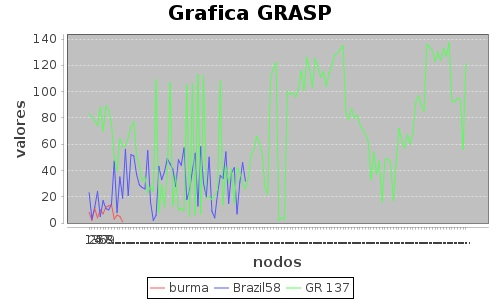
\includegraphics[width=12cm, height=9cm]{grafico.jpg}


\section{Inconvenientes con el tp}
\begin{enumerate}
  \item me costó plasmar lo que entendía en teoria a la práctica, me demoré mucho definiendo el dominio y redefiniendolo para poder codificar una solucion
  \item entendí las explicaciones que me dieron ante las consultas realizadas, pero pasarlo a codigo no me fue facil
  \item presentar la informacion en un grafico, me habia perdido en principio no sabia que valores debian tener los ejes x e y, luego de a poco transformar la informacion que disponia en puntos que entienda la herramienta graficadora me hizo realizar mas subtareas para que quede mas en claro que quise graficar´
\end{enumerate}
\section{Bibliografía}
\begin{itemize}
  \item Explicaciones de lo realizado en cada punto:
  
  Apuntes de cursada: Algoritmos - Universidad Nacional de Quilmes - 1er Semestre 2022
  \item Estilo y Formatos con LaTeX:
  
   http://minisconlatex.blogspot.com/2012/04/escribir-codigo-de-programacion-en.html
   \item Modelo de representacion de grafos, consultas varias:
   
   Libro de M.A.Weiss,“Estructuras de Datos en Java” 
   
   Libro de Luis Joyanes Aguilar
Ignacio Zahonero Martínez  “Estructuras de datos en Java”  
   
   \item Herramienta para dibujar el grafo:
   
   https://graphonline.ru/es/
\end{itemize}

\end{document}
